\documentclass[a4paper,12pt]{article}
\usepackage[french]{babel} 
\usepackage[T1]{fontenc}
%\usepackage[ansinew]{inputenc}
\usepackage[utf8]{inputenc}
\usepackage[top=3cm, bottom=3cm, left=2.3cm,right=2cm]{geometry}
\usepackage{graphicx}
\usepackage{color}
\usepackage{listings}
%\usepackage{marvosym}
%\usepackage{yfonts}
\usepackage[normalem]{ulem}
\usepackage{verbatim}
\usepackage{listings}
\usepackage{float}
%\renewcommand{\thesection}{\arabic{section}}
\usepackage{array} % pour les tableaux
\usepackage{amsmath} % pour les équations
\usepackage{float}
\usepackage{hyperref}	% crée des liens dans le pdf
\hypersetup{					% colorise les liens du pdf
  colorlinks=true,
  urlcolor=black
	citecolor=black,
  linkcolor=black,
  urlcolor=blue
}
\usepackage{url}			% change la police des url (utilisation : \url{http://asdf.ch})
\definecolor{dkgreen}{rgb}{0,0.6,0}
\definecolor{gray}{rgb}{0.5,0.5,0.5}
\definecolor{mauve}{rgb}{0.58,0.01,0.82}
%[babel=true]
\usepackage{csquotes}
\lstset{ %
  language=C,                % the language of the code
  basicstyle=\footnotesize,           % the size of the fonts that are used for the code
  numbers=left,                   % where to put the line-numbers
  numberstyle=\tiny\color{gray},  % the style that is used for the line-numbers
  stepnumber=1,                   % the step between two line-numbers. If it's 1, each line 
                                  % will be numbered
  numbersep=5pt,                  % how far the line-numbers are from the code
  backgroundcolor=\color{white},      % choose the background color. You must add \usepackage{color}
  showspaces=false,               % show spaces adding particular underscores
  showstringspaces=false,         % underline spaces within strings
  showtabs=false,                 % show tabs within strings adding particular underscores
  frame=single,                   % adds a frame around the code
  rulecolor=\color{black},        % if not set, the frame-color may be changed on line-breaks within not-black text (e.g. commens (green here))
  tabsize=2,                      % sets default tabsize to 2 spaces
  captionpos=b,                   % sets the caption-position to bottom
  breaklines=true,                % sets automatic line breaking
  breakatwhitespace=false,        % sets if automatic breaks should only happen at whitespace
  title=\lstname,                   % show the filename of files included with \lstinputlisting;
                                  % also try caption instead of title
  keywordstyle=\color{blue},          % keyword style
  commentstyle=\color{dkgreen},       % comment style
  stringstyle=\color{mauve},         % string literal style
  escapeinside={\%*}{*)},            % if you want to add a comment within your code
  morekeywords={*,...}               % if you want to add more keywords to the set
}


%en-tête
\usepackage{fancyhdr}
\lhead{CSEL}
\chead{}
\rhead{\today}
\pagestyle{fancy}

% Title Page
\title{\Huge{\textsc{Systèmes d'exploitation mobiles et applications}} \\ 
\Huge{\textbf{Miniprojet Android}\\\textbf{Sound Distance}} \\
\huge{Master HES-SO}}
\author{Émilie \textsc{Gsponer}, Grégory \textsc{Emery} }
\date{\today \\
version 1.0}

%-------------------------début du document-------------------------------------
\begin{document}

\maketitle % page de garde
\pagebreak
\tableofcontents % table des matières
\setlength\parindent{0pt}
\pagebreak
\section{But}
Créer une application mobile pour la mesure de distances basée sur la télémétrie par ultrasons. Réaliser des options pour des environnements ouverts ou avec des obstacles.
\section{Conception}
Nous avons choisi d'utiliser un module externe au téléphone mobile pour la mesure par ultrasons. Ce module est connecté à un Arduino munis d'un bloc de communication Bluetooth.\\
Nous avons donc une application sur smartphone qui communique par Bluetooth standard avec un Arduino équipé d'un module de télémétrie.
\begin{figure}[H]
	\begin{center}
		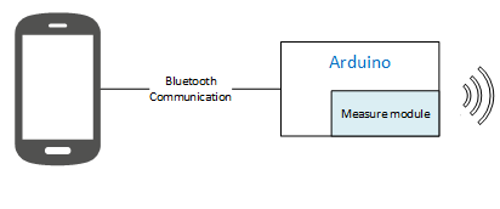
\includegraphics[width=10cm]{img/schemaBloc.png}
		\caption{Illustration de la communication}
		\label{schemabloc}
	\end{center}
\end{figure}
Ce projet à donc été séparé en deux parties distinctes, à savoir la programmation sur Android et celle sur Arduino.\\
Nous avons réaliser une première représentation de ce que nous voulions pour le projet.
\begin{figure}[H]
	\begin{center}
		\includegraphics[width=11.8cm]{img/concep0.png}
		\caption{Définition de la structure du projet}
		\label{conception0}
	\end{center}
\end{figure}
La partie "Arduino System" a été développé conformément au dessin avec les deux parties bluetooth et ultrasonic sensor.\\
Les différentes parties définies pour l'application Android ont été utilisées pour le développement. Nous avions décidé, dans un premier temps, d'utiliser divers capteurs comme l'accéléromètre et le compas pour avoir des informations sur l'orientation de la mesure, mais nous avons rejeté cette idée d'un commun accord avec notre professeur, car elle n'apportais pas grand chose aux mesures et compliquait l'interprétation des résultats.\\
Nous avions également dans l'idée de créer un boîtier pour l'Arduino avec le capteur à ultrason. Nous voulions faire en sorte que le smartphone puisse être intégré au boîtier. \\
Après réflexion, nous avons jugé plus judicieux de séparé l'Arduino du smartphone, car cela n'aurait pas été pratique pour prendre les mesures.\\\\
Sur cette base, nous avons été en mesure de respécifier les buts du projet. Nous allons donc réaliser une application Android permettant la mesure de distance par ultrason à l'aide d'un capteur externe sur Arduino. L'application servira uniquement à mesurer des espaces fermés comme des pièces de maison. On aura le choix entre trois types de mesure: une distance, une aire ou un volume.\\
Sur la base de ce cahier des charges, nous avons établis sur papier la représentation des différentes vues de l'application avec leur contenu et les informations passées entre elles. Nous nous sommes ensuite séparé le travail à réaliser.
\begin{figure}[H]
	\begin{center}
		\includegraphics[width=17cm]{img/concep1.png}
		\caption{Définition des différentes vues}
		\label{conception1}
	\end{center}
\end{figure}

\section{Réalisation}
L'application Android a été développé avec Android Studio et testé sur un Huawei P8 avec la version 5.0.1 d'Android et également sur Sony Xperia Z3 Compact. Le rendu de l'application n'est pas identique au niveau style sur les deux smartphones, mais le bon fonctionnement reste identique.\\
Le projet a permis d'acquérir des connaissances sur les points suivants:
\begin{enumerate}
	\item Découverte d'Android studio
	\item Définition de styles personnalisés
	\item ExpandableListView : Listes contenant des sous-catégories
	\item Communication Bluetooth standard
	\item Utilisation du synthétiseur vocale pour faire parler l'application
	\item Gestion d'un fichier dans la mémoire externe
	\item AlertDialog: Boîte de dialogue\\
\end{enumerate}

\subsection{Partie Arduino}
Concernant la partie Arduino, c'est une plateforme pour l'apprentissage et la réalisation de prototypes de systèmes électroniques. La carte électronique est accompagnée de deux petits circuits imprimés réalisant les fonctionnalités suivantes:
\begin{itemize}
	\item Carte HC-SR04, capteur de distance à ultrasons.
	\item Carte HC-05, carte bluetooth à connecter en UART à un module micro-contrôleur.
\end{itemize}
Pour que le système soit portable, une batterie alimente le tout.
\section{Problèmes rencontrés}
\section{Mode d'emploi}
\section{Conclusion}
Le développement de l'application s'est bien passé. Au début du projet, nous avons passé toute une après-midi à définir sur papier les différents écrans de l'application, leur organisation et contenu ainsi que les éléments passés entre les vues. Cette base nous a permis de bien nous répartir le travail à réaliser et à visualiser le résultat désiré.\\\\
Grégory s'est occupé de la programmation du Bluetooth sur l'Arduino ainsi que la gestion du module de mesure par ultrason. Il a également créer un boîtier pour la carte de mesure à l'aide d'une imprimante 3D. Il s'est également occupé, sur Android, de la création de la classe de mesure ainsi que de la vue gérant la prise de mesures. Dans cette partie il a utilisé le synthétiseur vocal du téléphone ainsi qu'une petite animation visuelle pour guider l'utilisateur.\\\\
Emilie a travaillé uniquement sur l'application Android. Elle a défini les différents styles pour les vues, créé la vue avec listant les mesures ainsi que celle permettant de les visualiser. Elle a également implémenté l'écran pour choisir le type de mesure à réaliser et s'est finalement occupée d'implémenter tout ce qui concerne la communication Bluetooth avec le module Arduino.\\\\
Nous sommes satisfaits de notre application, les objectifs que nous nous étions fixés ont été atteints. Nous voulions obtenir une application simple d'utilisation avec un design harmonieux entre les différentes vues. 




\end{document}


